%!TEX program = xelatex
\documentclass[a4paper, UTF8]{ctexrep}
\usepackage{ctex}
\usepackage{amsmath}
\usepackage{multirow}
\usepackage{amssymb}
\usepackage{graphicx}
\usepackage{geometry}
\usepackage{bm}
\usepackage{subfigure}
\usepackage{float}
\usepackage{array}
\usepackage{makecell}

\renewcommand\thesection{\arabic{section}}

\begin{document}
	\begin{titlepage}
		\centering
		\vspace{6cm}
		\LARGE{\textbf{Computer Vision HW1}}\\
		\vspace{4cm}
		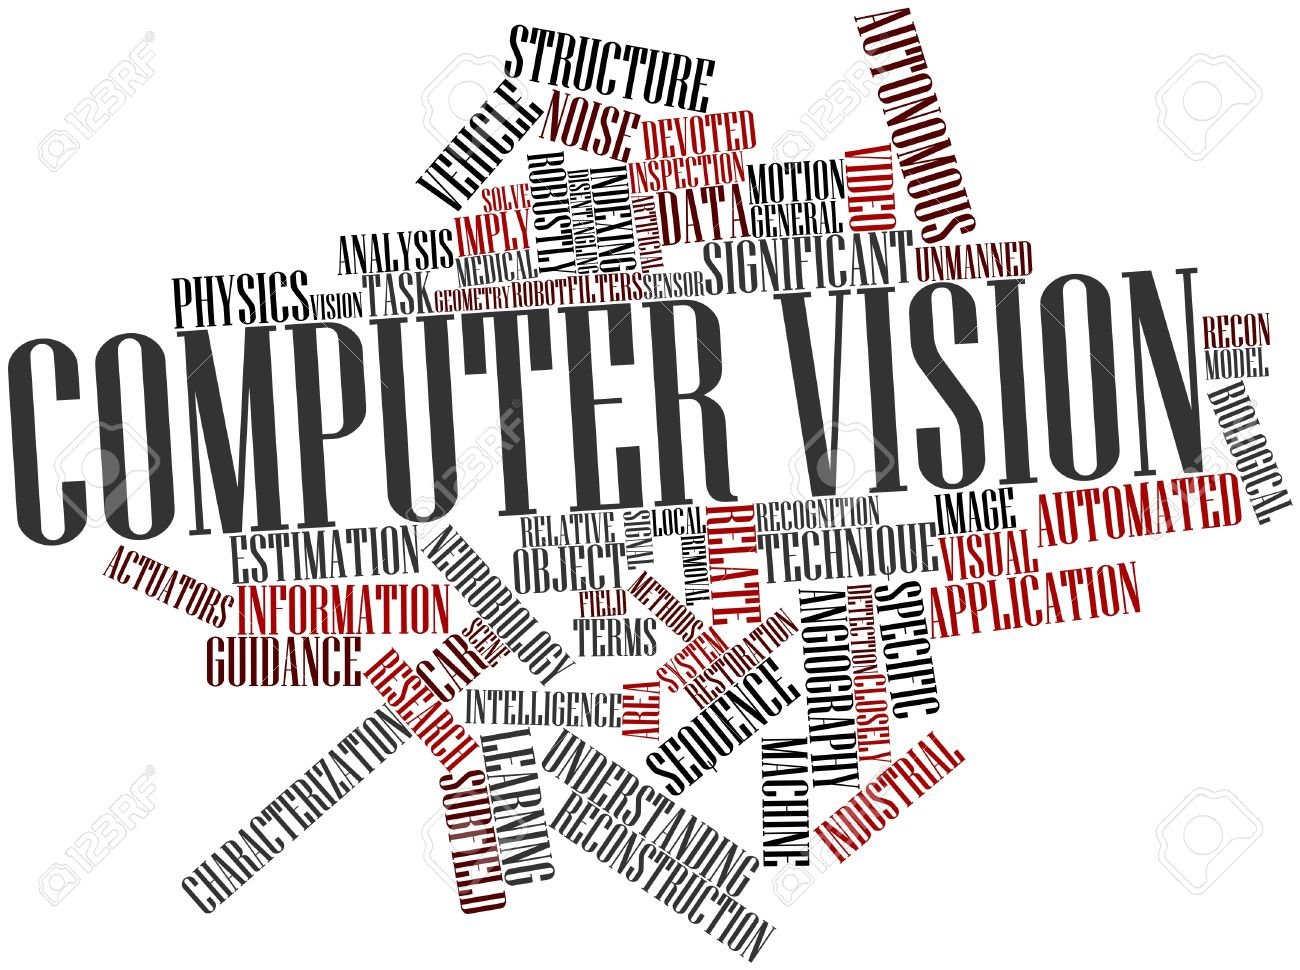
\includegraphics[width=0.8\textwidth]{cv.jpg}\\
		\vspace{5cm}
		\normalsize{安捷 1601210097}\\
		\normalsize{\today}
	\end{titlepage}
  \section{算法实现介绍}
    在这一次作业中,我按照作业要求,分别实现了Harris角点检测算法与SIFT特征检测与描述子生成算法,并针对作业中要求的具体问题,基于MATLAB编程实现了相关要求,其中,Harris角点检测算法我使用了MATLAB自带Harris角点检测函数;SIFT算子我使用了vl-feat工具包。
  \section{脚本功能介绍}
    为完成作业要求,我共编写三个MATLAB脚本,下面分别介绍其功能及对应的问题:
    \begin{description}
      \item[harris\_robustness\_test.m] 对应于作业的问题1,用于测试harris角点检测算法对于旋转、缩放的鲁棒性;
      \item[sift\_robustness\_test.m] 对应于作业的问题2,用于测试SIFT检测子对于图像旋转、缩放的鲁棒性;
      \item[sift\_descriptor\_robustness\_test.m] 对应于作业的问题3,用于测试SIFT描述子对于图像亮度、对比度、噪声、模糊的鲁棒性;
    \end{description}
  \section{各脚本参数设置}
    \subsection{harris\_robustness\_test.m参数设置}
      \begin{table}[htbp!]
        \centering
        \begin{tabular}{ccc}
        \hline
        参数名称 & 参数值 & 参数含义 \\
        \hline
        IMG\_PATH & 'cover\_1.jpg' & 图像路径 \\
        MIN\_QUALITY & 0.01 & Harris角点检测阈值 \\
        ROTATE\_ANGLE & 15 & 旋转角度 \\
        SCALE\_FACTOR & 1.2 & 缩放倍数 \\
        \hline
        \end{tabular}
        \caption{harris\_robustness\_test.m参数表}
      \end{table}

    \subsection{sift\_robustness\_test.m参数设置}
    \clearpage
      \begin{table}[htbp!]
        \centering
        \begin{tabular}{ccc}
        \hline
        参数名称 & 参数值 & 参数含义 \\
        \hline
        IMG\_PATH & 'cover\_1.jpg' & 图像路径 \\
        PEAK\_THRESH & 1 & SIFT算法峰阈值 \\
        EDGE\_THRESH & 5 & SIFT算法边阈值 \\
        ROTATE\_ANGLE & 15 & 旋转角度 \\
        SCALE\_FACTOR & 1.2 & 缩放倍数 \\
        \hline
        \end{tabular}
        \caption{sift\_robustness\_test.m参数表}
      \end{table}

    \subsection{sift\_descriptor\_robustness\_test.m参数设置}
      \begin{table}[htbp!]
        \centering
        \begin{tabular}{ccc}
        \hline
        参数名称 & 参数值 & 参数含义 \\
        \hline
        IMG\_PATH & 'building.jpg' & 图像路径 \\
        PEAK\_THRESH & 1 & SIFT算法峰阈值 \\
        EDGE\_THRESH & 5 & SIFT算法边阈值 \\
        ROTATE\_ANGLE & 15 & 旋转角度 \\
        SCALE\_FACTOR & 1.2 & 缩放倍数 \\
        BRIGHTNESS\_MINUS\_MAX & -100 & 最大亮度减小值 \\
        BRIGHTNESS\_PLUS\_MAX & 100 & 最大亮度增加值 \\
        BRIGHTNESS\_CHANGE\_LEVEL & 20 & 亮度增减幅度 \\
        CONTRAST\_MIN & 0.5 & 最小对比度调整值 \\
        CONTRAST\_MAX & 2.0 & 最大对比度调整值 \\
        CONTRAST\_CHANGE\_LEVEL & 0.25 & 对比度调整幅度 \\
        NOISE\_MIN & 0 & 最小高斯噪声标准差 \\
        NOISE\_MAX & 30 & 最大高斯噪声标准差 \\
        NOISE\_CHANGE\_LEVEL & 5 & 高斯噪声标准差调整幅度 \\
        GAUSS\_MIN & 1 & 最小高斯模糊标准差 \\
        GAUSS\_MAX & 10 & 最大高斯模糊标准差 \\
        GAUSS\_CHANGE\_LEVEL & 1 & 高斯模糊标准差调整幅度 \\
        \hline
        \end{tabular}
        \caption{sift\_descriptor\_robustness\_test.m参数表}
      \end{table}


  \section{软件版本及测试平台信息}
    这部分内容请参看源代码所在文件夹内的REAME文件。


\end{document}
